\chapter{研究内容}
\label{chap:contents}

本章では、本研究の内容を説明する。

\section{システム概要}

本システムはセンシングデータを個人でも簡単に利用できるようにすることが目的だ。
そのためのフレームワークを作成し、センシングデータを可視化するという二つの軸をもってシステムを構成した。

以下にシステムの構成を示す。大枠として、Linda\footnote{データをクラウド上で共有するためのフレームワーク。並列処理をしており、同時に多くのクライアントを処理できる。}からサーバーがデータを取得し、クライアントのリクエストに応じて送信する。クライアントでの情報は随時データベースに保存する。

\begin{table}[htbp]
  \caption{システム構成}
  \label{tb:files}
  \begin{center}\begin{tabular}{c|l}
    \hline
    システム&概要\\\hline\hline
    {\tt Linda}&データ元。データストリームからデータを取得する。\\\hline
    {\tt サーバー}&Lindaからデータを取得し、クライアントからのリクエストが来たら送信する。\\\hline
    {\tt クライアント}&サーバーにデータを要求し、ビジュアルプログラミングのビューを提供する。\\\hline
    {\tt データベース}&サーバー、クライアントのデータを保存している。\\\hline
  \end{tabular}\end{center}
\end{table}

\section{データの可視化}
センサーデータを二つの方法で可視化した。

まず一つ目として点滅によるデータの受信だ。Lindaから送られてきたデータを受信するとブロックが青に変化し、元に戻る。(図\ref{fig:image01})
センシングデータを監視してすぐにデータの受信に気付くことができるというメリットがある。\\

\begin{figure}[htbp]
  \begin{minipage}{0.5\hsize}
    \begin{center}
      \fbox{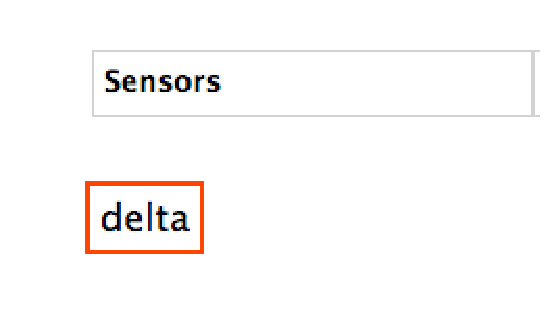
\includegraphics[width=50mm]{image/image1-1.eps}}
    \end{center}
  \end{minipage}
  \begin{minipage}{0.5\hsize}
    \begin{center}
      \fbox{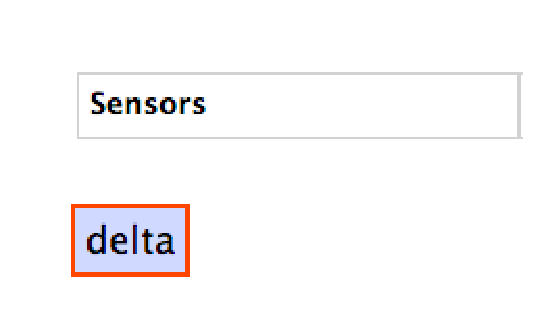
\includegraphics[width=50mm]{image/image1-2.eps}}
    \end{center}
  \end{minipage}
  \caption{点滅でのデータの通知}
  \label{fig:image01}
\end{figure}


そして二つ目として、実際の詳しいデータを見られるようにした。センサーオブジェクトに対してマウスオーバーしてフォーカスすることで実際の数字を表示できるようにした。(図\ref{fig:image02})

\begin{figure}[htbp]
    \begin{center}
       \fbox{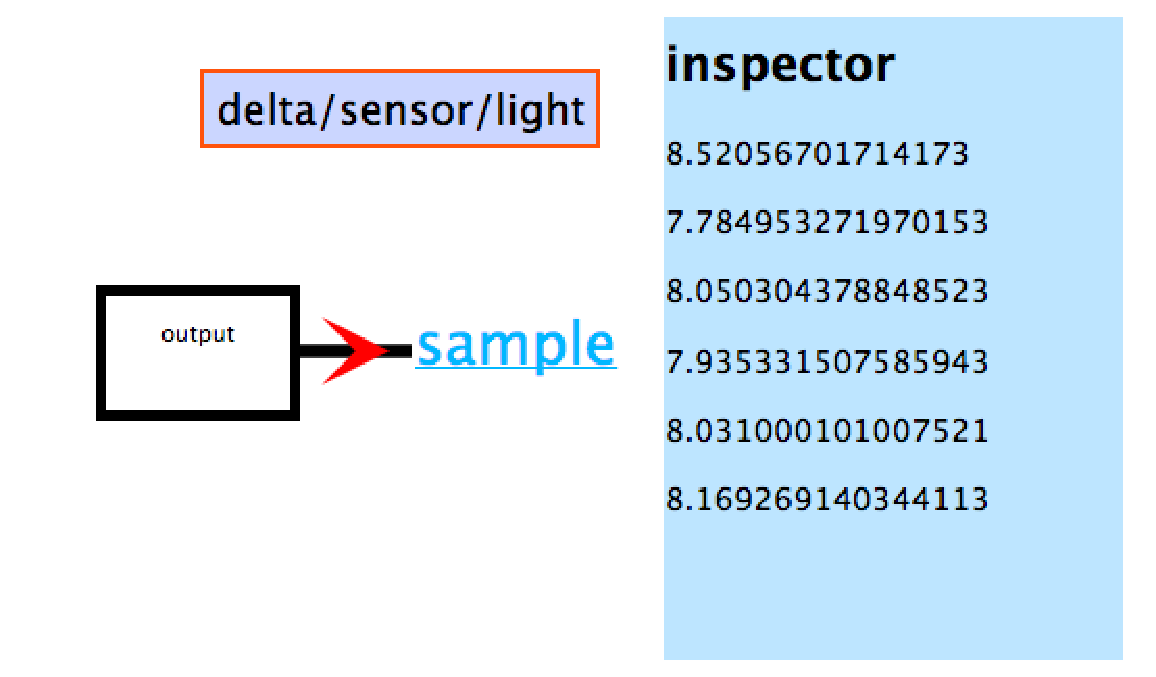
\includegraphics[width=100mm]{image/image02.eps}}
    \end{center}
    \caption{マウスオーバーによるデータの表示}
    \label{fig:image02}
\end{figure}

これら二つの実装により、センシングデータを閲覧する際に自分の欲しい粒度で取得することができるようになった。最低限の実装であれば詳しいデータが見られるだけでもいいが、抽象度を下げて色のみで表現することで閲覧する際の労力を下げることができる。

\section{ビジュアルプログラミング}

ビジュアルプログラミングを実装する際にブロック型のオブジェクトを作成した。以下にオブジェクトごとの解説をする。

\subsection{センサーオブジェクト}

ビジュアルプログラミングをする際には一番最初にセンサーオブジェクトを用意する。このオブジェクトはLindaからのデータを受信し、クライアント側でイベントを作成しデータを受信したら送信するというハブになっている。
また先に述べた通り、センサーデータが来るとこのブロックの点滅、あるいは能動的なデータの取得をすることが可能だ。

\subsection{条件オブジェクト}

センシングデータを扱うための条件オブジェクトを用意した。これにより上限下限、オンオフなどの条件分岐ができる。用意したオブジェクトを以下に列挙する。(図{\ref{fig:max}}〜図{\ref{fig:switch})これらのオブジェクトもブロックとして表現し、条件にマッチするとセンシングデータと同じように点滅する。

\begin{figure}[htbp]
  \begin{minipage}{0.5\hsize}
    \begin{center}
      \fbox{\includegraphics[width=50mm]{image/max.eps}}
    \end{center}
    \caption{Max: 最大値を設定}
    \label{fig:max}
  \end{minipage}
  \begin{minipage}{0.5\hsize}
    \begin{center}
      \fbox{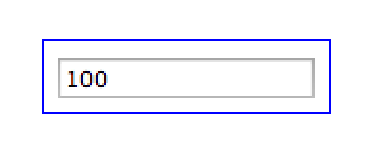
\includegraphics[width=50mm]{image/min.eps}}
    \end{center}
    \caption{min: 最小値を設定}
    \label{fig:min}
  \end{minipage}
\end{figure}

\begin{figure}[htbp]
  \begin{minipage}{0.5\hsize}
    \begin{center}
      \fbox{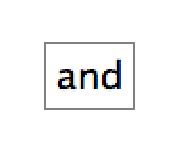
\includegraphics[width=50mm]{image/and.eps}}
    \end{center}
    \caption{and: 論理積を設定}
    \label{fig:and}
  \end{minipage}
  \begin{minipage}{0.5\hsize}
    \begin{center}
      \fbox{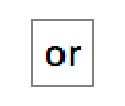
\includegraphics[width=50mm]{image/or.eps}}
    \end{center}
    \caption{or: 論理和を設定}
    \label{fig:or}
  \end{minipage}
\end{figure}

\begin{figure}[htbp]
  \begin{minipage}{0.5\hsize}
    \begin{center}
      \fbox{\includegraphics[width=50mm]{image/switch.eps}}
    \end{center}
    \caption{Switch: on/offを設定}
    \label{fig:switch}
  \end{minipage}
\end{figure}

\subsection{コネクションオブジェクト}

条件オブジェクトと同じ場所にあるが、その中で特殊なオブジェクトがコネクションオブジェクトである。コネクションオブジェクトはブロック間に親子件関係を作成できるオブジェクトである。

コネクションオブジェクトによって親のセンサーデータを条件オブジェクトの持つ自らの条件にかけ、次の世代に受け継ぐということが簡単にプログラムできるようになっている。

例えばdelta/sensor/lightからのセンサーデータかiota/sensor/lightからのセンサーデータがそれぞれ10以下でない場合にsampleというオブジェクトに通知を送るというような設定が簡単にできる。(図{\ref{fig:image03})

\begin{figure}[htbp]
    \begin{center}
       \fbox{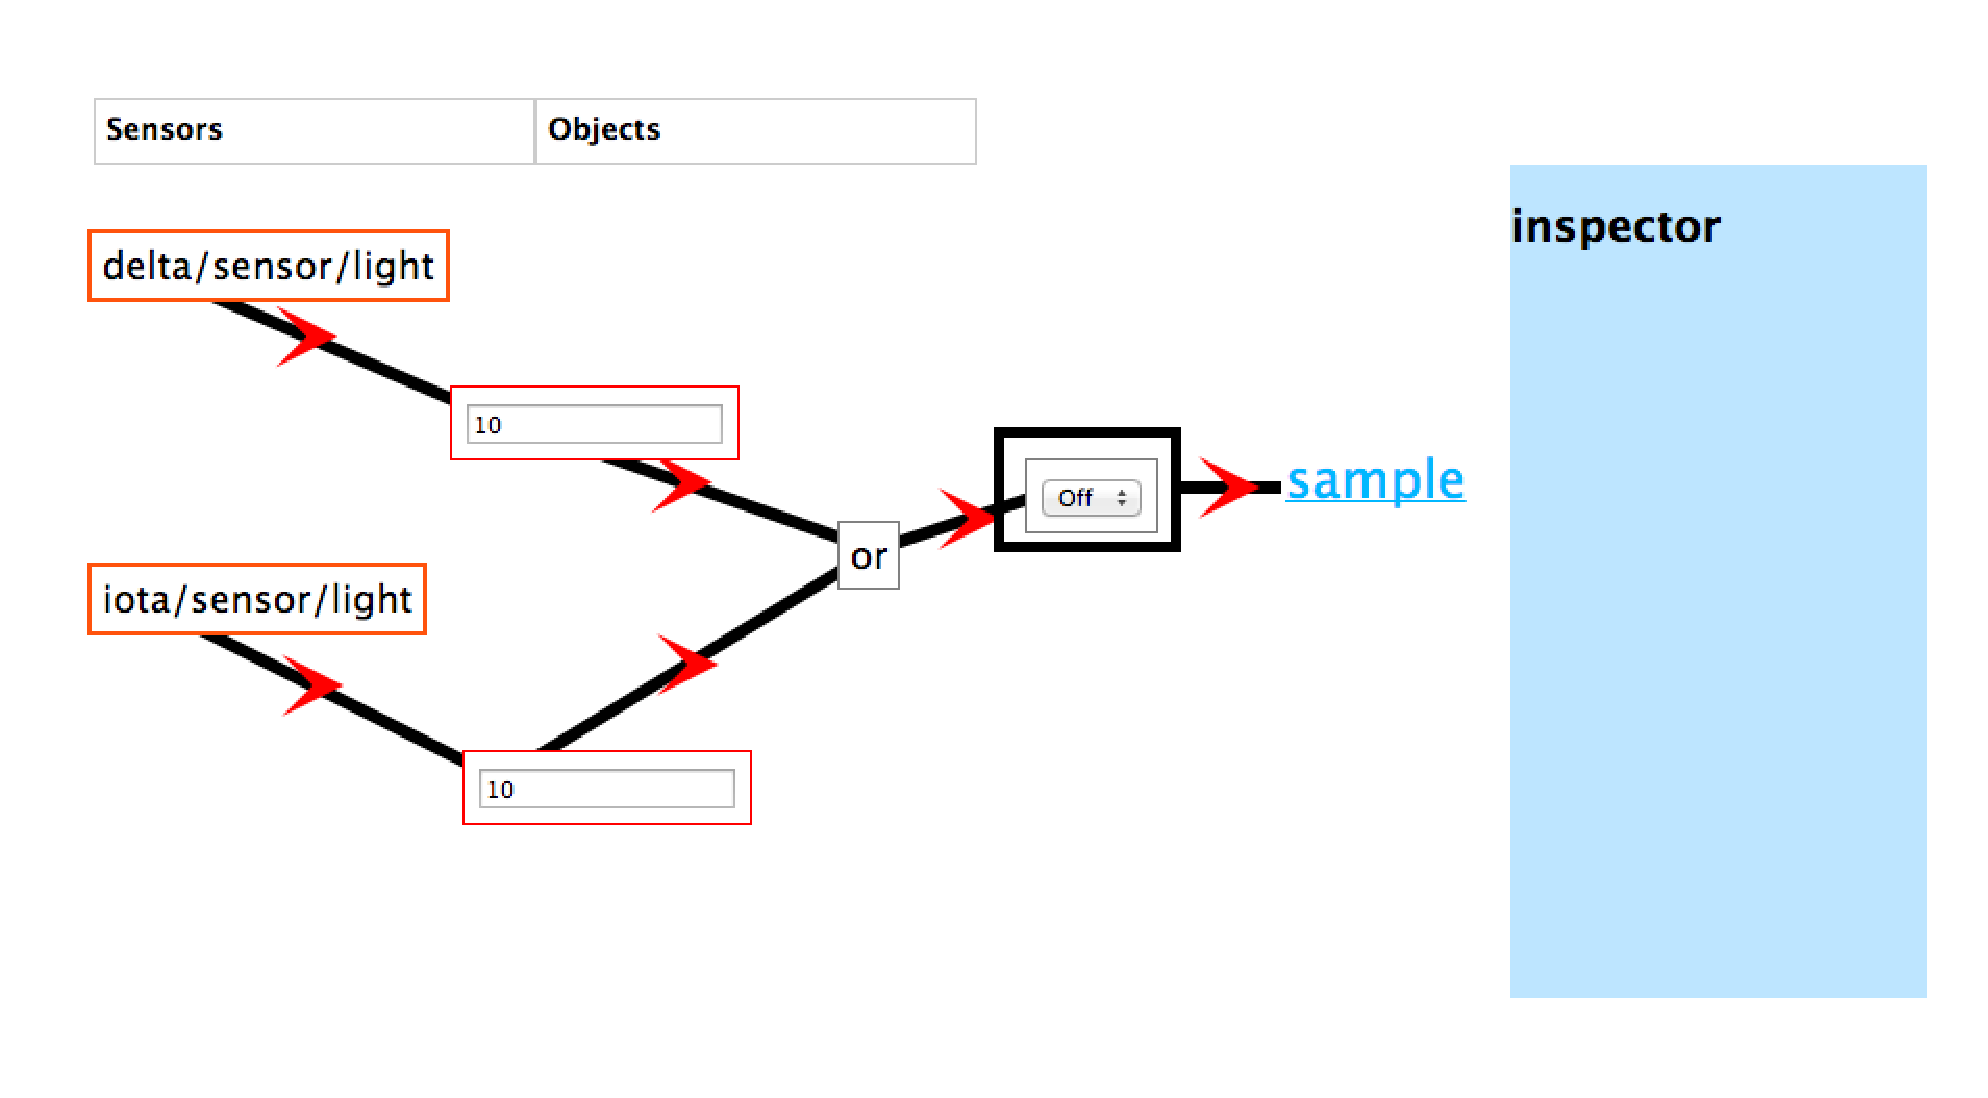
\includegraphics[width=150mm]{image/image03.eps}}
    \end{center}
    \caption{実際にセンシングデータをプログラミングする例}
    \label{fig:image03}
\end{figure}

\verb|\bibitem| コマンド中、参照用名称は、本文から参考文献を参照するときに使うので、忘れずに書いておく。参照文献を本文中に参照するときには、\verb|\cite{参照用名称}| のように書けばよい。例えば、この文の末尾には \verb|\cite{hoge09}| と書いてあるので、自動で対応する番号が振られる\cite{hoge09}\cite{hoge08}。
